\chapter{Introduction}

\label{chapter:intro}

Micro unmanned aerial vehicles (MAVs) recently saw a rise in usage across various fields. 
Drones are already widely used in cinematography \cite{Mademlis2020}, advertising \cite{Ullah2021} and agriculture \cite{Kim2019}. 
City emergency departments also use Unmanned arial vehicles (UAVs) - firefighters can use them to see and evaluate the situation from the sky, localize the source of fire and put it out \cite{Pritzl2021}.
Another field where UAVs can be used in nearest future is transportation. 
Fast parcel delivery \cite{San2018} and content transportastions \cite{Gupta2021,Aloqaily2022} are quite promissing fields of UAV application together with smart city comncept evolving \cite{Ortiz2019}.
Nowadays, even collaborative transportation systems are something non-fictional - swarms have become more popular, and that allows their usage for the transportation of really massive objects \cite{Bacelar2020} that one drone can not lift. 
UAVs and MAVs are also widely used in the military industry\cite{Duz2021}.

As drones are used so widely, they should become safer. 
Many commercially available drones are expensive and quite heavy, so accidents can be expensive and even cost somebody's life. 
Even if a drone is on remote control, the FOV of a pilot can not be more significant than the FOV of his eyes (which is about $130^\circ$), but dangerous obstacles can appear from any side.
In this sense, autonomous robots can see and avoid obstacles much better, but only if they have a well-designed system running onboard and enough sensors to cover the area around a drone.

Here is where safety systems become essential: if the only obstacles in the sky are birds, which usually are afraid of noise from UAVs, in a closed environment, in a forest or a city, there can be much more hindrances: trees, humans, other UAV's, falling or flying objects, furniture etc.
UAVs can have many sensors pointing in all directions to make themselves safe, and usually, they are not used in some closed environments due to their size.
For MAV, its size and weight can be obstructive, but they usually are used in a closed environment - they are small.
So it is always a tradeoff - the bigger UAV is, the more there may be sensors on it, and the bigger it should be to use it. 

Considering everything above, a compact obstacle avoidance system is a perspective field for research. 
Even though the idea is old, neither DJI, MRS, nor other research groups have a well-developed visual obstacle avoidance system. 
The best, for now, can be the Skydio system \footnotetext{\href{https://www.skydio.com/skydio-autonomy}{Skydio autonomy - https://www.skydio.com/skydio-autonomy }}, but their approach is for a forward-moving drone.

The inspiration for this project was taken from DJI's obstacle avoidance technology introduced with the release of the DJI Mavic 3 drone\footnote{\href{https://www.dji.com/cz/mavic-3}{DJI Mavic 3 - https://www.dji.com/cz/mavic-3}}. 
It uses visual data from monocular cameras with overlapping sones to cover almost the whole area around the UAV and react in real-time to obstacles nearby. 
Unfortunately, they have no publications or implementation details, so it is only a conclusion from publicly available information.

\section{Related Works}
Various MAVs use several obstacle avoidance sensors: stereo vision \cite{Ruf2018}, depth cameras (as Intel RealSense), monocular vision \cite{Mejias2010}, lidar (2d or 3d) \cite{Ramasamy2016}, sonar (ultrasonic), time of flight sensors, also combinations of them can be used. 
In \cite{Rambabu2015} the sensor fusion of ultrasonic and infrared sensors is presented.

Each of them has its pros and cons. 
3D lidars are more expensive than other sensors, but they can provide good accuracy, precision and 3d coverage of the envieronment; 2d lidars are successfully used for ground vehicles, but they are not so suitable for most tasks for MAVs because a car can be modelled as a 2 degrees of freedom (DoF) system, while MAVs always have 4DoF, some specialized even up to 6DoF. 
Depth cameras are more expensive than simple cameras. Ultrasonic and infrared sensors have distance limits and other minor issues ( a.e. sonar can be influenced by noise from the MAVs). 

In most articles stereo pair of two parallel cameras looking in the same direction is used (classical stereo pair) \cite{Yu2018, Lin2021, Xiao2019}, deep learning approaches \cite{Back2020, FragaLamas2019, Park2020, Roghair2021} and Convolutional Neural Networks \cite{Yu2013, Ma2020}. 
The real-time multi-camera feedback control system is introduced in \cite{He2021}, but this solution does not imply one drone, only multi-drone systems.

Real-time simultaneous localization and mapping (SLAM) systems can also be used for obstacle avoidance \cite{Moreno2014}. 
These problems are pretty closely related. 
SLAM keeps track of the robot's position while constructing and updating a map of an unknown environment; obstacle avoidance is a problem of detecting and avoiding the nearest obstacles in an unknown environment to keep drones safe.
So both problems are related to making a 3D map of an unknown environment, but for obstacle avoidance, the precision of distance measurements to the nearest objects is much more critical.

Structure from Motion (SfM) is another algorithm that can implement a system for avoiding obstacles. 
SfM is a method of depth map reconstruction from a continuous sequance of images, so using this approach, dense point clouds can be computed, and obstacles can be detected \cite{Lee2008}. 

\section{Problem definition}
\begin{figure}[t]
    \centering
    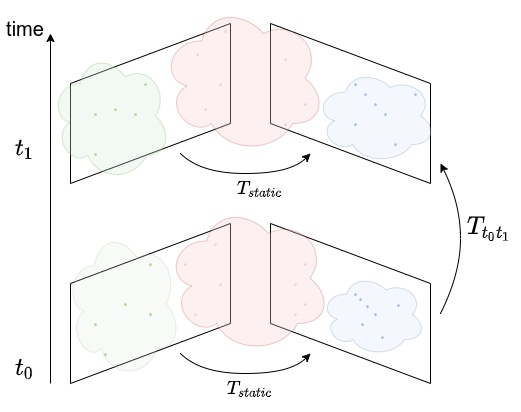
\includegraphics[width=0.7\textwidth]{graphics/general_scheme.png}
    \caption{General system scheme}
    \label{fig:intro_general}
\end{figure}

This thesis aims to design a visual obstacle avoidance system for MAVs, 3D model it, assemble a device and measure its efficiency. 
A working solution assumes a MAV with limited size and lifting force that limits the number of sensors on it; onboard setup of two calibrated (\autoref{sec:prelimin_calibration}) cameras with the known transformation between them.
Both cameras' FOV have an overlapping zone big enough to detect close obstacles.
Cameras' framerate guarantee system working in real-time (at least 30fps), and images from all cameras are synchronized in time.
Computational power is enough to make a system real-time.
MAV flies in an environment with some number of objects, such as an office or a room, to ensure that there is a sufficient number of features on images in a camera's overlapping sone for a feature detector, and it should calculate the distance to all surrounding objects with an allowable error.

On a figure \autoref{fig:intro_general} there is a scheme of a proposed system: $T_{static}$ is a transformation between cameras obtained after stereopair calibration. 
At each timestamp, new pair of images is received.
Feature detector extracts interesting points from the image, and then all points in a \textit{red} zone are filtered and matched.
It can be done because they are from an overlapping zone. 
In such a way, some 3d points are obtained already on a timestamp $t_0$. 
Then at a timestamp, $t_1$ new pair of images arrives - and the same process is repeated. 
Obtained point cloud can be used further to fix the scale of blue/green point clouds obtained from SfM and see the distance to objects that are not inside the overlapping zone.
It is also possible to use a red point cloud from $t_1$ as a starting point to apply the Iterative Closest Point algorithm to align red and blue points because red has common points.